\section{Key Components}

\subsection{Processor}
For this project, we'll be using a Zilog Z80 CPU. Why? Why not! It's one of the classic processors from the early home computer days (being found in the Radio Shack TRS-80 line, the ZX Spectrum and other Sinclair Research computers, and as a co-processor in many, many other systems, not to mention as the heart of many classic arcade games). While one could debate the merits of the Z80 vs. the 6502 vs. whatever other older processor you want to pick - and arguably, the 6502 is a strong processor and a popular choice - we're going to take the Z80 as our decision and more forward. The concepts we learn here can be applied to any of these other processors should you wish to use on in your own design.

It does appear that the Z80 is easier to find online for sale, and at a lower price, which doesn't hurt. 

The Z80 comes in many variants. We are specifically using Z80 part number \textbf{Z0840004PSC}, which means that our version of the Z80 has some specific traits:

\begin{itemize}
\item The processor is designed to run at speeds up to 4Mhz.
\item The processor is packaged in a 40 pin Dual Inline Package (DIP), which makes breadboarding and building our computer much easier than working with other IC package types.
\item The processor is built on NMOS technology, which will become important when we determine the components to interface to the processor.
\item The item is the "commercial" variant of the Z80. This is in contrast to the "industrial" and "military" versions, which are hardened to withstand harsher environments.
\end{itemize}

Otherwise, it's a Z80, so its method of operation, instruction set, etc. is the same as any other Z80 chip. For example, Jameco (www.jameco.com), as of this writing, sells new the 6Mhz version of this chip (Jameco part number 35705). They also have a CMOS variant that runs at 2.5MHz (Jameco part number 35561). If you can't find the exact part number I am using, any of these variants is fine\footnote{The 2.5MHz CMOS version is actually quite attractive; it is less expensive and requires less power.}. The key is the packaging and the logic level, which we are expecting to be +5V / TTL compatible. 

\subsubsection{The Z80 Datasheet}

How can we be sure if the Z80 we are using is appropriate? That it is a +5V device with TTL compatible logic levels? The vendor should have the datasheet available for the specific part you are looking at, and in that datasheet you will look for a section called "DC Characteristics". From that section, I've extracted part of the relevant table (the table in the datasheet will have more rows that what I am showing here):


\resizebox{\textwidth}{!}{%
\begin{tabular}{|c|l|c|c|c|c|l|}
\hline
\multicolumn{7}{|l|}{$V_{cc}$ $5V$ $\pm 5\%$ unless otherwise specified}\\
\hline
\textbf{SYMBOL} & \textbf{PARAMETER} & \textbf{MIN.} & \textbf{TYP.} & \textbf{MAX.} & \textbf{UNIT} & \textbf{TEST CONDITION} \\
\hline
$V_{ILC}$ & Clock Input Low Voltage & $-0.3$ & & $0.8$ & $V$ & \\
\hline
$V_{IHC}$ & Clock Input High Voltage & $V_{cc} - 0.6$ & & $V_{cc} + 0.3$ & $V$ & \\
\hline
$V_{IL}$ & Input Low Voltage & $-0.3$ & & $0.8$ & $V$ & \\
\hline
$V_{IH}$ & Input High Voltage & $2.0$ & & $V_{cc}$ & $V$ & \\
\hline
$V_{OL}$ & Output Low Voltage & & & $0.4$ & $V$ & $I_{OL} = 1.8mA$ \\
\hline
$V_{OH}$ & Output High Voltage & $2.4$ & & & $V$ & $I_{OH} = -250\mu A$ \\
\hline
\end{tabular}}

There are four pieces of information to note, and which ensure us that the part we are looking at meets our expectations:

\begin{itemize}
\item The $V_{cc}$ listing at the top indicates that the primary power for the process is $5V$, which is what we are designing our circuit around
\item The $V_{ILC}$ and $V_{IHC}$ numbers tell us what is expected for the incoming clock signal. A low value is execpted to be between $-0.3V$ and $0.8V$, which is in line with a TTL low level. The high is expected to be between $4.4V$ and $5.3V$ (based on $V_{CC} = 5V$), which is high but within the realm of a TTL level. We will need to remember that the clock is expecting high to be at least $4.4V$, not $2.0V$ which would otherwise be the bare minimum TTL HIGH.
\item The $V_{IL}$ and $V_{IH}$ indicate what our input logic levels should be. Low is between $-0.3V$ and $0.8V$, while high is between $2.0V$ and $5V$ - exactly what we expect it to be. 
\item Correspondingly, $V_{OL}$ and $V_{OH}$ are the low and high logicl levels the chip will output, and which again are in the expected TTL range\footnote{The standard output logic high voltage for TTL is $2.7$, not $2.4$, but since any TTL device must treat anything at $2.0$ or higher as high, this is still fine.}.
\end{itemize}

OK - so we have selected a processor, and we know the basics of how that processor will interface (5V TTL) with the rest of our components. 

\chapter{Expirements}
\section{Standing Up the Z80}

Let's start this process by making sure we can get our Z80 processor to work properly. Building incrementally, and learning as we go,
is key to how we are approaching the creation of our Retro Computer. Following a similar approach will be helpful for you as you explore new components and systems of your own design.

We want to minimize the number of failure points, so we are going to take our first steps with the Z80 using the Arduino as our bootstrap. We know we are working with a +5V processor expecting TTL-level logic signals, so the Arduino will interface without having to do any special level shifting. What we need to do is to ascertain the \textit{bare minimum} we need to do to the Z80 to make it function (and, of course, we need some way of confirming that the processor \textit{is} doing something!).

What's the simplest thing we can have the Z80 do? Without any memory, we can't provide the Z80 with any kind of interesting program to run. Without any I/O devices, we can't enter data or see the results of any program anyway. Instead, we will \textit{trick} the Z80 into thinking it is reading a program from memory - but it will be the world's most boring program, and endless series of NOP instructions.

NOP stands for \textit{no operation}. It's an instruction that effectively does nothing, other than to tell the processor to move on to the next instruction. An endless series of of NOPs will cause the processor to run forever, doing 'nothing' but looking at memory address after memory address, finding NOP after NOP. What helps us out here is that the binary code for NOP is 00000000.

We don't have to build any kind of memory into this exiprement; we simply need to ensure that whenever the Z80 tries to read from memory looking for an instruction, that all of the data lines are 0. It will think it has read from memory and found a NOP.

Since the Z80 will execute the NOP then move to the next address, we can check to see if the Z80 is working by looking at the address bus. If we connect some LED's to the bus, we should see them turn on and off in an ascending binary pattern every few clock ticks (it takes the Z80 multiple clock ticks to execute an instruction).

Reviewing the datasheet, we see have a number of pins on the Z80 that we will need to do something with:

\resizebox{\textwidth}{!}{%
\begin{tabular}{|c|c|l|}
\hline
\textbf{Pin} & \textbf{Name} & \textbf{Notes} \\
\hline
$A_{0}$ - $A_{15}$ & Address Bus & We will use the address bus to view the actions of the processor. \\
\hline
$D_{0}$ - $D_{7}$ & Data Bus & We need to tie these low to simulate a NOP instruction. \\
\hline
$M_{1}$ & Machine Cycle One & This is an output pin, which we can ignore. \\
\hline
$MREQ$ & Memory Request & This is an output pin, which we can ignore. \\
\hline
$IORQ$ & Input/Output Request & This is an output pin, which we can ignore. \\
\hline
$RD$ & Memory Read & This is an output pin, which we can ignore. \\
\hline
$WR$ & Memory Write & This is an output pin, which we can ignore. \\
\hline 
$REFSH$ & Refresh & This is an output pin, which we can ignore. \\
\hline
$HALT$ & Halt & This is an output pin, which we can ignore. \\
\hline
$WAIT$ & Wait & We need to turn this pin off or the Z80 will enter into a waiting state. \\
\hline
$INT$ & Interrupt Request & We need to turn this input pin off. \\
\hline
$NMI$ & Non-Maskable Interrupt & This also needs to be turned off. \\
\hline
$RESET$ & Reset & We will need to temporarily activate this pin to get the Z80 started properly. \\
\hline
$BUSRQ$ & Bus Request & Another input pin that needs to be turned off. \\
\hline
$BUSAK$ & Bus Acknowledge & This is an ouput pin, which we can ignore. \\
\hline
$CLK$ & Clock & We need to provide a clock signal to the Z80. \\
\hline
\end{tabular}}

\begin{center}
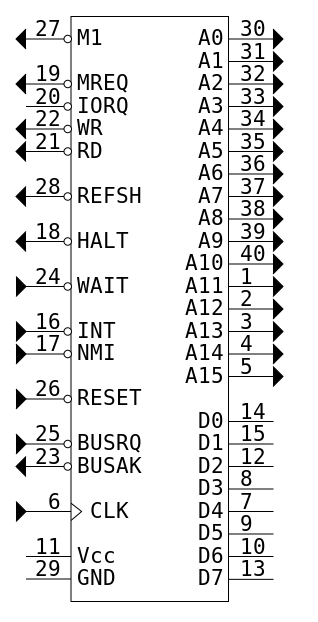
\includegraphics[height=6cm]{Z80_pinout.png}
\end{center}

Some comments:

\begin{itemize}
\item The WAIT, INT, NMI and BUSRQ pins are \textbf{active low}. This means that the pin's logic levels are effectively inverted; a 'low' is ON or 1, a 'high' is OFF or 0. To turn these pins off, we must actually provide +5V. 
\item The Data Bus is not inverted; it is \textbf{active high}. With any IC, though, we can't leave an input pin unconnected and just assume that it will be a zero (the Data Bus are tri-state, input/output pins). We need to explicitly set it low, which we do by connecting the pin to ground through a small resistor.
\end{itemize}

It looks like there are a number of pins we can either safely ignore, or simply tie to either +5V or ground. And although we didn't list them, we do need to provide +5V of power and make a ground connection. 
